\documentclass{report}
\usepackage{amsmath}
\usepackage{ngerman}
\usepackage[hidelinks]{hyperref}
\usepackage[numbered]{bookmark}
\usepackage{pgfplots}
\usepackage{listings}
\usepackage{color}
\usepackage{attachfile}

\usetikzlibrary{positioning,matrix, arrows.meta}

\pgfplotsset{compat=1.18}
\tracinglostchars=2

\definecolor{dkgreen}{rgb}{0,0.6,0}
\definecolor{gray}{rgb}{0.5,0.5,0.5}
\definecolor{mauve}{rgb}{0.58,0,0.82}

\lstset{
    frame=tb,
    language=Java,
    aboveskip=3mm,
    belowskip=3mm,
    showstringspaces=false,
    columns=flexible,
    basicstyle={\small\ttfamily},
    numbers=none,
    numberstyle=\tiny\color{gray},
    keywordstyle=\color{blue},
    commentstyle=\color{dkgreen},
    stringstyle=\color{mauve},
    breaklines=true,
    breakatwhitespace=true,
    tabsize=4
}

\title{\textbf{Informatik-Abitur}}
\author{Tim Teichmann}
\date{\today}

\begin{document}
\maketitle
\tableofcontents

\chapter{Datenstrukturen}
\begin{flushleft}   
    Datenstrukturen speichern Daten, damit später ohne Probleme auf diese Daten zugegriffen werden kann.
    Man nennt sie Daten\textbf{\textit{strukturen}}, da die Daten, die gespeichert werden auf eine bestimmte Art und Weise angeordnet (strukturiert) werden.
\end{flushleft}

\section{Statisch}
\begin{flushleft}
    Statische Datenstrukturen sind -- wie der Name schon sagt -- bestimmt.
    Sie sind relativ fest angeordnet und können schlecht bis gar nicht verändert werden.
\end{flushleft}

\subsection{Array}
\begin{flushleft}
    Arrays sind im Prinzip Listen, die eine feste Größe haben.
    Sie speichern Elemente eines Typs.
    Das bedeutet, dass ein einzelnes Array nicht dafür gedacht ist Integer und Strings zu speichern. \\
    Um Arrays vernünftig zu verstehen sieht man hier ein Beispiel für ein Array, das Integer speichert:
\end{flushleft}

\begin{center}
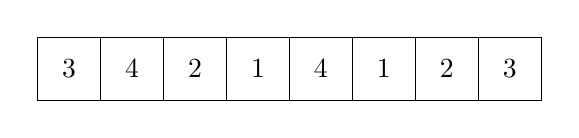
\begin{tikzpicture}
    \matrix (A) [matrix of nodes, nodes={draw, minimum size=8mm},column sep=-\pgflinewidth]{
        3 & 4 & 2 & 1 & 4 & 1 & 2 & 3 \\
    };
\end{tikzpicture}
\end{center}

\begin{flushleft}
    Arrays weisen jedem Element, das sie speichern einen \textit{Index} zu.
    Indices (Mehrzahl eines Index) starten in der Regel bei $0$.
    Das erste Element des Beispiel-Arrays hat den Wert $3$ und liegt beim Index $0$.
    Hier ein Beispiel zur Erstellung und Nutzung eines Arrays in Java.
    \begin{lstlisting}
        // Array.java
        
        // Unser Beispiel-Array erstellen
        int[] array = {3,4,2,1,4,1,2,3};

        // Die Laenge unseres Beispiel-Arrays abrufen
        int arrLen = array.length;
        
        // Den Wert des ersten Elements (3) in die Variable firstElem speichern
        int firstElem = array[0];

        // Ein Array erstellen, das vier mal den Wert 0 speichert
        int[4] array1;
    \end{lstlisting}
\end{flushleft}

\section{Dynamisch}
\begin{flushleft}   
    Dynamische Datenstrukturen sind -- vorallem im Vergleich zu statischen Datenstrukturen -- agil.
    Es ist sehr viel leichter Elemente zu entfernen oder hinzuzufügen, da die Größe von dynamischen Datenstrukturen nicht fest ist.
\end{flushleft}

\subsection{Queue}
\subsubsection{Einführung}

\begin{flushleft}   
    Queue bedeutet übersetzt Warteschlange oder Schlange.
    Genau nach diesem Prinzip funktioniert auch eine Queue. \\
    Ein Mensch stellt sich in eine Schlange hinter andere Menschen.
    Vor ihm werden viele Leute aufgerufen, bis er dran kommt.
    Jede Person in der Warteschlange wird nacheinander abgearbeitet.
    Die erste Person, die sich anstellt, wird auch als erstes aufgerufen. \\
    Das nennt man auch \textit{First-In-First-Out} (\textit{FIFO}) Prinzip.
    Hier ein Bild zu der Erklärung:
\end{flushleft}

\begin{center}
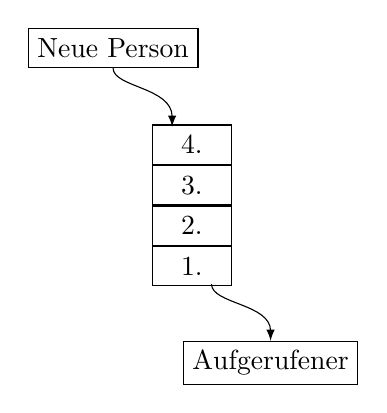
\begin{tikzpicture}[draw,minimum width=1cm,minimum height=0.5cm]
    \node[draw] (in) at (-1,2) {\text{Neue Person}};
    \node[draw] (out) at (1,-2) {\text{Aufgerufener}};
    \matrix (queue)[matrix of nodes,nodes={draw, nodes={draw}}]{
         4. \\ 3. \\ 2. \\ 1. \\
     };

    \draw[-latex] (0.25,-1) .. controls (0.25,-1.25) and (1,-1.25) .. (out.north);
    \draw[-latex] (in.south) .. controls (-1,1.5) and (-0.25,1.5) .. (-0.25,1);
\end{tikzpicture}
\end{center}

\begin{flushleft}
    Das Aufrufen einer Person, entfernt diese aus der Queue.
    Dieser Prozess wird auch \textit{dequeue} genannt.
    Wenn sich eine neue Person anstellt, wird sie der Queue hinzugefügt.
    Das nennt man \textit{enqueue}. \\
    Weitere typische Operationen einer Queue sind:
    \begin{enumerate}
        \item {
                Das erste Element einer Queue aufrufen mit \textit{front}
            }
        \item {
                Prüfen ob die Queue leer ist mit \textit{isEmpty}
            }
    \end{enumerate}
    Eine allgemeine Queue würde also so aussehen:
\end{flushleft}

\begin{center}
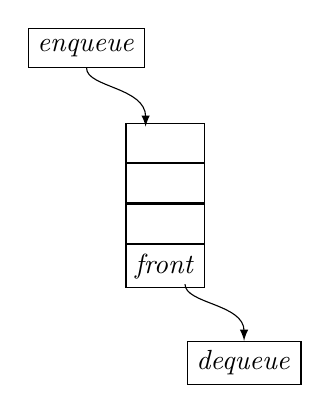
\begin{tikzpicture}[draw,minimum width=1cm,minimum height=0.5cm]
    \node[draw] (in) at (-1,2) {\textit{enqueue}};
    \node[draw] (out) at (1,-2) {\textit{dequeue}};
    \matrix (queue)[matrix of nodes,nodes={draw, nodes={draw}},nodes in empty cells]{
        \\ \\ \\ \textit{front} \\
    };

    \draw[-latex] (0.25,-1) .. controls (0.25,-1.25) and (1,-1.25) .. (out.north);
    \draw[-latex] (in.south) .. controls (-1,1.5) and (-0.25,1.5) .. (-0.25,1);
\end{tikzpicture}
\end{center}

\begin{flushleft}
    Im Abitur wird eine Queue als Java-Klasse vorgegeben. \\
    \href{https://raw.githubusercontent.com/tim-tm/informatik-notes/main/code/Queue.java}{\textit{Abiturvorgabe: Queue}}
\end{flushleft}

\subsubsection{Anwendung}
\begin{flushleft}
    Für Queues gibt es meistens immer ähnliche Aufgaben: \\
    Einfache Queues:
    \begin{lstlisting}
        // Erstellt eine Queue von Strings
        Queue<String> queue = new Queue<>();
        
        // Fuegt der Queue eine neues Element mit dem Wert "Hallo" hinzu
        queue.enqueue("Hallo");

        // Gibt das erste Element der Queue ("Hallo") in der Konsole aus
        System.out.println(queue.front());

        // Entfernt das erste Element ("Hallo") aus der Queue
        queue.dequeue();
    \end{lstlisting}
    \href{https://raw.githubusercontent.com/tim-tm/informatik-notes/main/code/Queue_Beispiel1.java}{\textit{Unkommentierter Code}} \\
    Queues mit eigenen Klassen:
    \begin{lstlisting}
        // Unsere eigene Klasse um Koordinaten zu speichern
        class Koordinate {
            int x;
            int y;
        }
        
        // Erstellt eine Queue von Koordinaten
        Queue<Koordinate> queue = new Queue<>();
        
        // Wir moechten eine neue Koordinate hinzufuegen
        // 1. Die Koordinate erstellen
        Koordinate coord = new Koordinate();
        
        // 2. Werte fuer x und y setzen
        coord.x = 100;
        coord.y = 150;

        // 3. Die Koordinate der Queue hinzufuegen
        queue.enqueue(coord);
    
        // Die erste Koordinate ausgeben
        // 1. Die Koordinate aus der Queue holen
        Koordinate koord = queue.front();

        // 2. X-Wert der Koordinate ausgeben
        System.out.println(koord.x);
        
        // 3. Y-Wert der Koordinate ausgeben
        System.out.println(koord.y);

        // Erste Koordinate (x=100, y=150) aus der Queue entfernen
        queue.dequeue();
    \end{lstlisting}
    \href{https://raw.githubusercontent.com/tim-tm/informatik-notes/main/code/Queue_Beispiel2.java}{\textit{Unkommentierter Code}} \\
    Bei diesem Beispiel fällt vorallem auf, dass plötzlich viel mehr Schritte benötigt werden um ein Element hinzuzufügen.
    Das kann vereinfacht werden indem man der Klasse einen \textit{Konstruktur} gibt.
    Der \textit{Konstruktor} wird ausgeführt wenn man ein neues Objekt der Klasse erstellt.
    \begin{lstlisting}
        // Unsere eigene Klasse um Koordinaten zu speichern
        class Koordinate {
            int x;
            int y;
            
            /** 
                * Diese besondere Methode (Konstruktur) wird aufgerufen, wenn wir new Koordinate() ausfuehren.
                * Unsere Variablen x und y sollen zu den neuen Werten, also unseren Parametern xNeu und yNeu gesetzt werden.
                * Achtung: Der Name des Konstruktors muss genau mit dem Namen der Klasse uebereinstimmen.
                */
            public Koordinate(int xNeu, int yNeu) {
                x = xNeu;
                y = yNeu;
            }
        }
        
        // Erstellt eine Queue von Koordinaten
        Queue<Koordinate> queue = new Queue<>();
        
        // Wir moechten eine neue Koordinate hinzufuegen
        // 1. Die Koordinate erstellen
        // Anstatt unsere Werte fuer x und y erst nach dem Erstellen einzutragen, packen wir diese jetzt einfach direkt in die Klammern, wenn wir unsere Koordinate erstellen.
        // Das funktioniert nur, weil wir in der Definition unserer Klasse einen Konstruktor erstellt haben.
        Koordinate coord = new Koordinate(100, 150);

        // 2. Schritt faellt weg

        // 3. (jetzt 2.) Die Koordinate der Queue hinzufuegen
        queue.enqueue(coord);
    
        // Ausgeben und entfernen bleibt gleich
    \end{lstlisting}
    \href{https://raw.githubusercontent.com/tim-tm/informatik-notes/main/code/Queue_Beispiel3.java}{\textit{Unkommentierter Code}} \\
    Dadurch, dass wir einen Konstruktor erstellt haben, sparen wir uns jedes mal wenn wir ein Objekt erstellen zwei Zeilen code. \\
    Kompliziertere Aufgaben mit Queues:
    \begin{lstlisting}
        /*
            * 1. 
            *      Die Aufgabenstellung sagt uns, dass es bereits eine Queue namens queue gibt, diese speichert Strings.
            *      Wir sollen jedes Element dieser Queue entfernen und ausgeben lassen.
            */

        // Die Schleife wird durchlaufen, solange es noch Elemente in der Queue gibt.
        // Also solange sie nicht leer ist (!isEmpty).
        while (!queue.isEmpty()) {
            // Das erste Element der Queue in der Variable s speichern
            String s = queue.front();

            // Die Variable s, also das erste Element der Queue ausgeben lassen
            System.out.println(s);

            // Das erste Element (hier: s) aus der Queue entfernen
            // Ohne diesen Schritt wuerde die Schleife unendlich lange das erste Element ausgeben
            queue.dequeue();
        }
    \end{lstlisting}
    \href{https://raw.githubusercontent.com/tim-tm/informatik-notes/main/code/Queue_Beispiel4.java}{\textit{Unkommentierter Code}} \\
\end{flushleft}

\subsection{Stack}
\subsubsection{Einführung}

\begin{flushleft}
    Die deutsche Übersetzung für ein Stack ist: Stapel.
    Das sind Stacks auch, ein Stapel auf den man Dinge legen, oder von dem man Dinge nehmen kann.
    Stacks funktionieren nach dem \textit{Last-In-First-Out} (\textit{LIFO}) Prinzip.
    Man kann also immer nur das letzte Element, was auf den Stapel gelegt wurde wieder vom Stapel nehmen.
    Typische Operationen sind:
    \begin{enumerate}
        \item {
                \textit{push} - Elemente hinzufügen
            }
        \item {
                \textit{pop} - Elemente entfernen
            }
        \item {
                \textit{top} - Auf das oberste Element zugreifen
            }
        \item {
                \textit{isEmpty} - Prüfen ob der Stack leer ist
            }
    \end{enumerate}
    So kann man sich einen Stack vorstellen:
\end{flushleft}

\begin{center}
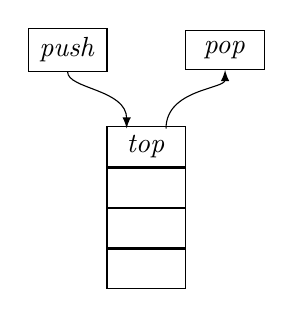
\begin{tikzpicture}[draw, minimum width=1cm, minimum height=0.5cm]
    \node[draw] (in) at (-1,2) {\textit{push}};
    \node[draw] (out) at (1,2) {\textit{pop}};
    \matrix (queue)[matrix of nodes, nodes={draw, nodes={draw}}, nodes in empty cells]
    {
        \textit{top} \\ \\ \\ \\
    };

    \draw[-latex] (0.25,1) .. controls (0.25,1.5) and (1,1.5) .. (out.south);
    \draw[-latex] (in.south) .. controls (-1, 1.5) and (-0.25,1.5) .. (-0.25,1);
\end{tikzpicture}
\end{center}

\begin{flushleft}
    Wie bei der Queue wird im Abitur eine Java Stack Klasse vorgegeben:
    \href{https://raw.githubusercontent.com/tim-tm/informatik-notes/main/code/Stack.java}{\textit{Abiturvorgabe: Stack}} \\
\end{flushleft}

\subsubsection{Anwendung}

\end{document}
